\setcounter{chapter}{1}
\chapter{Orientação a Objetos com JavaScript}

\begin{flushright}
	\textit{
		Dedique-se aos estudos para que eles o façam \\
		melhor para a sociedade e para si mesmo.
	} \\
	
	\textbf{Alvaro Granha Loregian}
\end{flushright}

Esse capítulo tem como objetivo aplicar o conhecimento adquirido anteriormente no Capítulo \ref{cap:cap1} utilizando a linguagem de programação JavaScript. 

JavaScript, segundo \citeonline{fernandotrasviña2021}, tem fortes capacidades de programação orientada a objetos, apesar de ocorrerem algumas discussões devido às diferenças da orientação a objetos no JavaScript em comparação com outras linguagens. Assim, no Capítulo \ref{cap:cap1} foi realizada uma introdução à programação orientada a objetos, e neste, será demonstrado os conceitos de programação orientada a objetos no JavaScript.

\section{Classes}

Classes em JavaScript\footnote{Para mais detalhes acesse: \url{https://developer.mozilla.org/pt-BR/docs/Web/JavaScript/Reference/Classes}} são introduzidas no ECMAScript\footnote{Para mais detalhes acesse: \url{https://developer.mozilla.org/pt-BR/docs/Web/JavaScript}} 2015 e são simplificações da linguagem para as heranças baseadas nos protótipos. A sintaxe para classes não introduz um novo modelo de herança de orientação a objetos em JavaScript. Classes em JavaScript provêm uma maneira mais simples e clara de criar objetos e lidar com herança.

\begin{figure}[H]
	\centering
	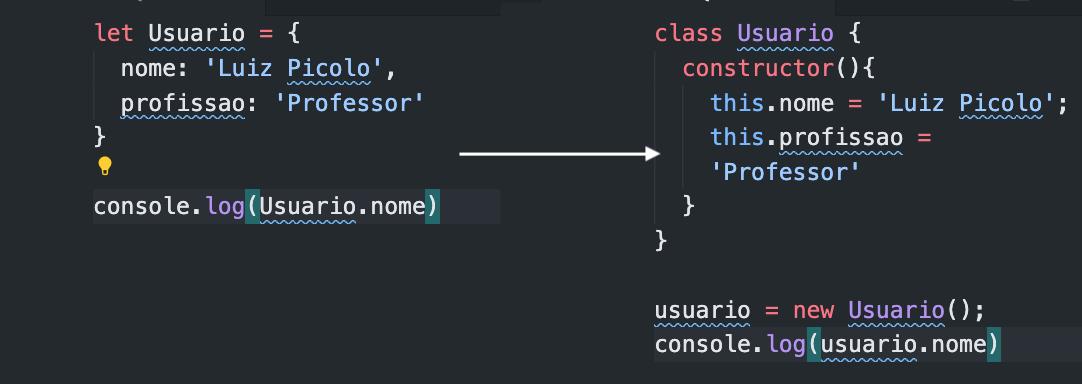
\includegraphics[scale=0.35]{imagens/classes-antes-depois.png}
	\caption{Sintaxes de classes em JavaScript}
	\legend{Fonte: O Autor }
	\label{fig:sintaxe-classe-js}
\end{figure}

Para definir uma classe é usando uma declaração de classe. Para declarar uma classe, deve-se usar a palavra reservada \textbf{class} seguida pelo nome da classe desejada.

\begin{minted}[frame=single,framesep=10pt,breaklines,linenos,tabsize=2]{javascript}
	class Retangulo {
	
	}
\end{minted}

Outras forma de escrita de uma classe, também chamadas Expressões de Classes (\textit{class expression}), podem ser usadas para fazer sua definição. Contudo, utilizaremos apenas a notação mais nova e comumente encontrada em outras linguagens, ou seja, a notação \textit{class}.

\begin{minted}[frame=single,framesep=10pt,breaklines,linenos,tabsize=2]{javascript}
	// sem nome
	let Retangulo = class {
		
	};
	
	// nomeada
	let Retangulo = class Retangulo {
		
	};
\end{minted}

E para que possamos criar uma instância (objeto) da classe, utilizamos o seguinte trecho de código abaixo.

\begin{minted}[frame=single,framesep=10pt,breaklines,linenos,tabsize=2]{javascript}
	let retangulo = new Retangulo();
\end{minted}

\section{Construtor e Atributos}

Como dito no Capítulo \ref{cap:cap1} as características que descrevem um objeto são chamadas na orientação a objeto de atributos. Assim, toda classe pode conter atributos que lhe dão as características necessárias para a criação do objeto. 

Para que possamos criar nossos atributos podemos fazer de duas formas, uma usando funções diretas ou por meio do Construtor. Um contrutor é um tipo especial de ``método'' para criar e iniciar um objeto criado pela classe. Só pode existir um método construtor dentro da classe. Um erro de sintáxe \textbf{SyntaxError} será lançado se a classe possui mais do que uma ocorrência do método construtor. 

Para iniciarmos os atributos com o construtor usamos a palavra reservada \textbf{constructor} seguida dos valores dos atributos desejados.

\begin{minted}[frame=single,framesep=10pt,breaklines,linenos,tabsize=2]{javascript}
	class Retangulo {
	  constructor(altura, largura) {
	  	this._altura = altura;
	  	this._largura = largura;
	  }
	}
\end{minted}

\section{Métodos}

% https://developer.mozilla.org/pt-BR/docs/Web/JavaScript/Reference/Classes	
Métodos são ações que o objeto pode realizar e são responsáveis pela troca de mensagem entre os objetos \textbf{emissores} e o \textbf{receptores}. As técnicas de programação orientada a objetos recomendam que a estrutura de um objeto e a implementação de seus métodos devem ser tão privativos como possível. Normalmente, os atributos de um objeto não devem ser visíveis externamente. Da mesma forma, de um método deve ser suficiente conhecer apenas sua especificação, sem necessidade de saber detalhes de como a funcionalidade que ele executa é implementada\footnote{Veja mais em: \url{https://www.devmedia.com.br/orientacao-a-objetos-parte-ii/7161}}.

\begin{figure}[H]
	\centering
	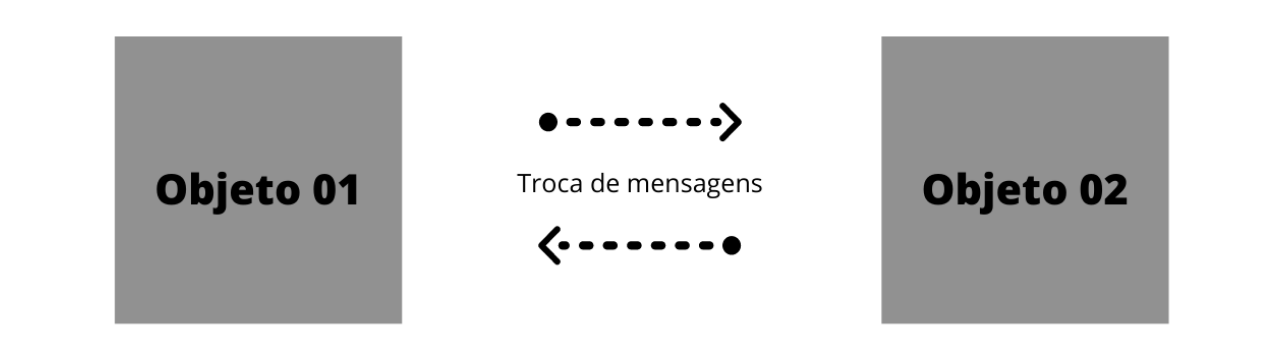
\includegraphics[scale=0.5]{imagens/troca-mensagens.png}
	\caption{Troca de mensagens entre objetos.}
	\legend{Fonte: O Autor }
	\label{fig:troca-mensagem}
\end{figure}

Assim, para definir um método, devemos atribuir uma função a uma classe que, depois disso, poderá ser chamado como método do objeto usando o mesmo nome ao qual foi atribuída a função. 

\begin{minted}[frame=single,framesep=10pt,breaklines,linenos,tabsize=2]{javascript}
	class Retangulo {
		constructor(altura, largura) {
			this._altura = altura;
			this._largura = largura;
		}
	
		calcularArea() {
			return this._altura * this._largura;
		}
	}
\end{minted}

Para invocarmos o método, basta instânciar-mos a classe e criar assim um novo objeto.

\begin{minted}[frame=single,framesep=10pt,breaklines,linenos,tabsize=2]{javascript}
	const objeto = new Retangulo(10, 10);
	console.log(objeto.calculaArea());
\end{minted}

Contudo, existe aqui um erro semântico. Quando queremos saber a área de uma figura geométrica, deveríamos ``perguntar'' a está figura sua área e não solicitar o calculo. Logo, podemos resolver isso, criando um novo método que retorna apenas a área e que utiliza o método \textbf{calcularArea}. 

\begin{minted}[frame=single,framesep=10pt,breaklines,linenos,tabsize=2]{javascript}
	class Retangulo {
		constructor(altura, largura) {
			this._altura = altura;
			this._largura = largura;
		}
	
		area(){
			return this.calcularArea();
		}
		
		calcularArea() {
			return this._altura * this._largura;
		}
	}

	const objeto = new Retangulo(10, 10);
	console.log(objeto.area());
\end{minted}

\subsection{Método Get}

Os métodos criados acima funcionam corretamente. Porém, podemos melhorar um pouco mais a semântica do objeto. Para isso usaremos a sintáxe \textbf{Get}.

Às vezes é desejável que se permita acesso a uma propriedade que retorna um valor computado dinamicamente, ou você pode querer refletir o status de uma variável interna sem requerer o uso de chamadas de método explícitas. Em Javascript, isso pode ser feito com o uso de um \textbf{getter}. Não é possível simultaneamente ter um \textbf{getter} associado a uma propriedade e a mesma possuir um valor, embora seja possível usar um \textbf{getter} e um setter em conjunto para criar algo como uma pseudo-propriedade.

\begin{minted}[frame=single,framesep=10pt,breaklines,linenos,tabsize=2]{javascript}
	class Retangulo {
		constructor(altura, largura) {
			this._altura = altura;
			this._largura = largura;
		}
		
		get area(){
			return this.calcularArea();
		}
		
		calcularArea() {
			return this._altura * this._largura;
		}
	}
	
	const objeto = new Retangulo(10, 10);
	console.log(objeto.area);
\end{minted}

\subsection{Método Set}

Já o \textbf{setter} pode ser usado para executar uma função sempre que se tenta mudar uma propriedade específica. \textbf{Setters} são geralmente usados em conjunto com \textbf{getters}, para criar um tipo de pseudo-propriedade. No entanto é impossível ter-se um \textbf{setter} para uma propriedade que contenha um valor real.

\begin{minted}[frame=single,framesep=10pt,breaklines,linenos,tabsize=2]{javascript}
	class Retangulo {
		
		set altura(altura){
			this._altura = altura;
		}
		
		set largura(largura){
			this._largura = largura;
		}
		
		get area(){
			return this.calcularArea();
		}
		
		calcularArea() {
			return this._altura * this._largura;
		}
	}
	
	const objeto = new Retangulo();
	objeto.largura = 10;
	objeto.altura = 10;
	console.log(objeto.area);
	
	objeto.largura = 100;
	objeto.altura = 100;
	console.log(objeto.area);
\end{minted}

O setter se torna muito útil nesse caso pois não precisaremos criar uma novo objeto, apenas alteramos seus atributos (seu estado) para obter novos valores.

\subsection{Método Static}

A palavra chave \textbf{static} define um método estático para a classe. Métodos estáticos não são chamados na instâncias da classe. Em vez disso, eles são chamados na própria classe. Geralmente, são funções utilitárias, como funções para criar ou clonar objetos. Chamadas a métodos estáticos são feitas diretamente na classe e não podem ser feitas em uma instância da classe. Métodos estáticos são comumente utilizados como funções utilitárias\footnote{Veja mais em: \url{https://developer.mozilla.org/pt-BR/docs/Web/JavaScript/Reference/Classes/static}}.

\begin{minted}[frame=single,framesep=10pt,breaklines,linenos,tabsize=2]{javascript}
	class Retangulo {
		
		// Codigo anterior
		
		// Metodo adicionado
		static formaGeometrica(objeto){
			if (objeto._altura == objeto._largura){
				return ``A forma geometrica é um Quadrado''
			} else {
				return ``A forma geometrica é um Retangulo''
			}
		}
	}
	
	const objeto = new Retangulo();
	objeto.largura = 10;
	objeto.altura = 10;
	console.log(Retangulo.formaGeometrica(objeto));
	console.log(objeto.area);
\end{minted}

\section{Exercícios de fixação}

\begin{enumerate}
	\item Uma empresa de notícias \textbf{IFNews} necessita desenvolver um portal de notícias. Após criada toda a parte documental, você, que é desenvolvedor/desenvolvedora na empresa, deverá iniciar a criação dos primeiros códigos. Sua primeira tarefa é a criação da classe Noticia. A classe deverá ser codificada seguindo, primordialmente, as definições abaixo: 
	
	\begin{enumerate}
		\item \textbf{Nome da classe}: Noticia
		\item \textbf{Atributos}: Título, Data da Publicação, Resumo e Texto (Outros atributos podem ser adicionados)
		\item \textbf{Métodos:} Mostrar Noticia (Outros métodos podem ser adicionados)
	\end{enumerate}

	Ao instanciar a classe e invocar o método \textbf{mostrar notícia} o resultado final deverá ser semelhante ao descrito abaixo (Lembre-se que o conteúdo no título, a data e o texto dependerá do \textbf{estado} adicionado a seu objeto): 
\end{enumerate}

\textbf{Resultado esperado:} 

\begin{figure}[H]
	\centering
	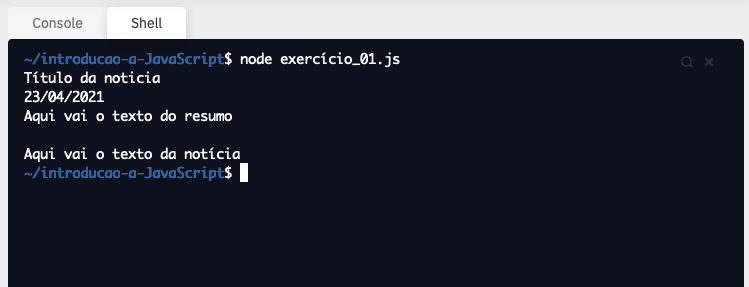
\includegraphics[scale=0.5]{imagens/saida-exer-01.png}
	\caption{Resultado esperado}
	\legend{Fonte: O Autor }
	\label{fig:resultado}
\end{figure}

\section{Exercícios extras}

\begin{enumerate}
	\item Crie uma classe para representar uma \textbf{pessoa}, com os atributos \textbf{nome, data de nascimento e altura}. Crie o método \textbf{constructor} para inicializar os atributos e também um método para imprimir todos dados de uma pessoa e outro para calcular a idade.

	\item Crie uma classe para representar um \textbf{jogador de futebol}, com os atributos \textbf{nome, posição, data de nascimento, nacionalidade, altura e peso}. Crie o método para imprimir todos os dados do jogador. Crie um método para calcular a idade do jogador e outro método para mostrar quanto tempo falta para o jogador se aposentar. Para isso, considere que os jogadores da posição de defesa se aposentam em média aos 40 anos, os jogadores de meio-campo aos 38 e os atacantes aos 35.

	\item Escreva uma classe cujos objetos representam alunos matriculados em uma disciplina. Cada objeto dessa classe deve guardar os seguintes dados do aluno: matrícula, nome, 2 notas de prova e 1 nota de trabalho. Escreva os seguintes métodos para esta classe:

	\begin{itemize}
		\item \textbf{media:} calcula a média final do aluno (cada prova tem peso 2,5 e o trabalho tem peso 2) 
		\item \textbf{final:} calcula quanto o aluno precisa para a prova final (retorna zero se ele não for para a final)
	\end{itemize}
	
	\item Crie uma classe Agenda que pode armazenar 10 pessoas e que seja capaz de realizar as seguintes operações:

	\textbf{armazena(nome, idade, altura);} \\
	\textbf{remove(nome);} \\
	\textbf{busca(nome);} // informa em que posição da agenda está a pessoa \\
	\textbf{imprimeDadosAgenda();} // imprime os dados de todas as pessoas da agenda \\
	\textbf{mostrar(index);} // imprime os dados da pessoa que está na posição ``i'' da
agenda. 
\end{enumerate}

\section{Herança}

A definição de herança, já abordada no Capítulo anterior, nós diz que: a herança é uma maneira de reutilizar código a medida que podemos aproveitar os atributos e métodos de classes já existentes para gerar novas classes mais específicas que aproveitarão os recursos da classe hierarquicamente superior \cite{evandroeduardoseronruiz2008}.

Para realizar a reutilização ja citada, no ES6 foi adicionada a palavra reservada \textbf{\textit{extends}}. Uma classe pode herdar atributos e métodos de outra classe por meio da extensão da classe desejada. 

\begin{minted}[frame=single,framesep=10pt,breaklines,linenos,tabsize=2]{javascript}
class Retangulo {
	
	// Codigo anterior
	...
}

class Quadrado extends Retangulo{
	constructor(lado) {
		super(lado, lado);
	}
}

let objeto = new Quadrado(100)
console.log(objeto.area)
\end{minted}

Observem a palavra \textbf{super}. A palavra reservada \textbf{super} é usada para acessar o objeto pai de um objeto, em outros casos, é usada para acessar a classe pai de uma classe. Neste caso, precisamos observar alguns pontos: 

\begin{itemize}
	\item No construtor, o \textbf{super} deve ser chamado antes de qualquer acesso à \textbf{this};
	\item Caso a classe que está realizando \textit{extends} não defina o constructor ele será definido e chamado implicitamente passando todos os parâmetros.
\end{itemize}

\begin{minted}[frame=single,framesep=10pt,breaklines,linenos,tabsize=2]{javascript}
// Errado
class Quadrado extends Retangulo{
	constructor(lado) {
		this._lado = lado;
		super(lado, lado);
	}
}

// Correto
class Quadrado extends Retangulo{
	constructor(lado) {
		super(lado, lado);
		this._lado = lado;
	}
}
\end{minted}

\section{Super classe e Subclasse}

Atrelado com o conceito de herança possuímos as definições de \textbf{Super classe} e \textbf{Subclasses}.  O uso da palavra \textbf{extends} indica que a classe deveria ser baseado em um objeto padrão. Isso é chamado de Super Classe (\textbf{\textit{superclass}}) e a classe derivada é a Subclasse (\textbf{\textit{subclass}}) \cite{haverbeke2018eloquent}

\begin{minted}[frame=single,framesep=10pt,breaklines,linenos,tabsize=2]{javascript}
class Retangulo {
   ...
}

class Quadrado extends Retangulo{
   ...
}
\end{minted}

Ocasionalmente, é útil saber se um objeto foi derivado de uma
classe. Para isso, o JavaScript fornece um operador binário chamado \textbf{instanceof} \cite{haverbeke2018eloquent}. 

\begin{minted}[frame=single,framesep=10pt,breaklines,linenos,tabsize=2]{javascript}
console.log(new Quadrado(2) instanceof Retangulo) \\ True
\end{minted}

Mas e \textbf{Retangulo} é instância de alguma classe? Neste caso sim, todos os objetos em javaScript herdam a classe pai nomeado de \textbf{Object}

\begin{minted}[frame=single,framesep=10pt,breaklines,linenos,tabsize=2]{javascript}
	console.log(new Quadrado(2) instanceof Object) \\ True
	console.log(new Retangulo(2, 2) instanceof Object) \\ True
\end{minted}

\section{Exercícios de fixação}

\begin{enumerate}
	\item A empresa de notícias \textbf{IFNews} contratou você para desenvolver o portal de notícias, o qual teve seu início no exercício anterior. Sua primeira tarefa foi a criação da classe Noticia que possuía as seguintes definições: 
	
	\begin{enumerate}
		\item \textbf{Nome da classe}: Noticia
		\item \textbf{Atributos}: Título, Data da Publicação, Resumo e Texto (Outros atributos podem ser adicionados)
		\item \textbf{Métodos:} Mostrar Noticia (Outros métodos podem ser adicionados)
	\end{enumerate}
\end{enumerate}

Após desenvolver a tarefa, a empresa criou uma nova solicitação. O portal deve possuir \textbf{notícias em destaque}, as quais devem conter uma imagem seguida de um título e um resumo. Como você já criou uma notícia que contem parte do que o cliente necessita, a única tarefa será criar uma \textbf{subclasse} que herdará as características e ações da \textbf{Super Classe} e adicionará a característica desejada.

	\begin{enumerate}
	\item \textbf{Nome da classe}: NoticiaDestaque
	\item \textbf{Atributos}: ImagemDestaque (apenas o caminho da imagem)
	\item \textbf{Métodos:} Mostrar Destaque (Outros métodos podem ser adicionados)
\end{enumerate}

\textbf{Resultado esperado:} 

\begin{figure}[H]
	\centering
	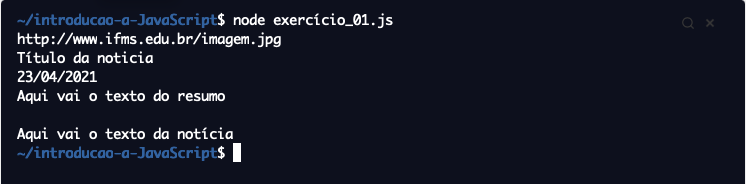
\includegraphics[scale=0.5]{imagens/exercicio_heranca.png}
	\caption{Resultado esperado}
	\legend{Fonte: O Autor }
	\label{fig:resultado2}
\end{figure}

\section{Exercícios extras}

\begin{enumerate}
	\item Crie classes de forma a representar o diagrama a abaixo:
	
	\begin{figure}[H]
		\centering
		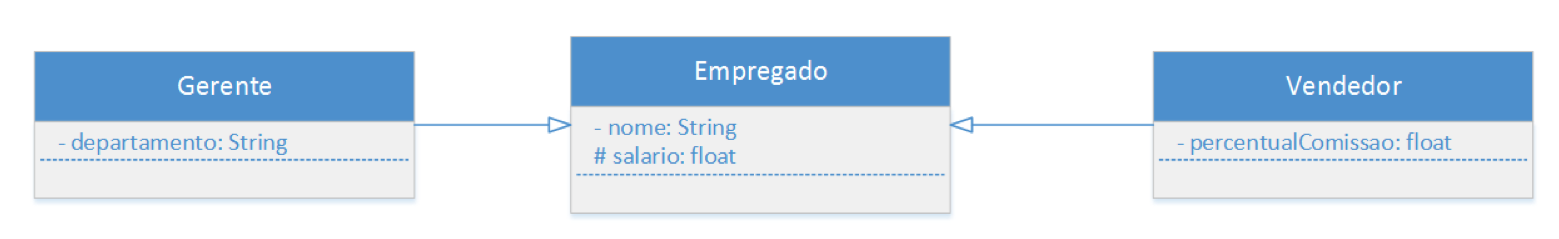
\includegraphics[scale=0.3]{imagens/exercicio-fix-02-01.png}
	\end{figure}
\end{enumerate}


\section{Tratamento de erros}

Um requisito de software que deveríamos priorizar, em qualquer projeto, é como vamos realizar o tratamento de erros e exceções da nossa aplicação. 
\textbf{Saber como gerenciar erros é parte importante da programação.}

Existem dois tipos básicos de erros na programação:

\begin{itemize}
	\item Erros de sintaxe;
	\item Erros de tempo de execução;
\end{itemize}

\subsection{Erros de sintaxe}
Os erros de sintaxe, também conhecidos como erros de análise, no tempo de interpretação no \textit{JavaScript} (Linguagem interpretada / Linguagem compilada). Esse erro ocorre porque ao digitarmos algum código errado, ou seja, no momento em que esquecemos parênteses ou chaves, etc.	
	
\begin{minted}[frame=single,framesep=10pt,breaklines,linenos,tabsize=2]{javascript}
class Retangulo { 
	constructor(altura, largura){
		this._altura = altura;
		this._largura = largura;
	}	
	// Falta fechar as chaves
\end{minted}
		
Ao executar o código acima, o retorno será: \textbf{SyntaxError: Unexpected end of input}

Os erros de Sintaxe são erros mais simples de serem resolvidos. Existem algumas maneiras de evitar esses tipos de erros, as quais são:

\begin{itemize}
	\item Verificar o seu código e procurá-los (não é eficaz e pode levar muito tempo)
	\item Outra opção é usar alguma ferramenta ou plugin IDE. (eslint , jshint e jslint)
\end{itemize}

Essas ferramentas são muito populares e os(as) desenvolvedores(as), não gostam de tarefas repetitivas.


\subsection{Erros de tempo de execução}
Erros de execução, também chamados de \textbf{exceções}, ocorrem durante a execução (após a compilação/interpretação). Este tipo de erro não impede a compilação ou interpretação de um código. Contudo, o código gerado não funcionará.

\begin{minted}[frame=single,framesep=10pt,breaklines,linenos,tabsize=2]{javascript}
class Retangulo { 
	constructor(altura, largura){
		this._altura = altura;
		this._largura = largura;
	}	
}

let retangulo = new Retangulos(); // Nome no plural
\end{minted}

Ao executar o código acima, o retorno será: \textit{ReferenceError: Retangulos is not defined}

Por esse ser um erro mais complexo de ser tratado algumas linguagens implementam alguns mecanismos interessantes para manipular o retorno dos erros, sendo que, as exceções são utilizadas como uma forma de \textit{feedback}, para que o(a) desenvolvedor(ar) possa saber o que fazer quando cair numa situação de erro. 

Assim, para capturar estes erros e aplicar algum tratamento, podemos usar a sintaxe \textbf{try} \textbf{catch} a qual será o assunto a seguir.

\subsection{Sintaxe do Try Catch Finally}

A sintaxe do \textbf{try} \textbf{catch} é composta por dois blocos principais:
\begin{itemize}
	\item O \textit{try} é o local na qual o código é executado 
	\item O \textit{catch}, e o local que você recebe, via parâmetro na função, um \textbf{objeto do tipo Error}. 
\end{itemize}

\begin{minted}[frame=single,framesep=10pt,breaklines,linenos,tabsize=2]{javascript}
try {
	// seu codigo aqui
} catch (error) {
	// tratamento de erro aqui
}
\end{minted}

\subsection{Sintaxe do Try / Catch / finally}	
Nós podemos também usar a cláusula \textbf{finally}. Este bloco será executado sempre independente se houver ou não falha. Depois que o \textit{try} ou \textit{catch} serem executados, este bloco será acionado. 

Isto pode ser útil por exemplo, para fechar um arquivo que foi aberto para leitura, registrar algum log ou fechar alguma conexão. Veja a sintaxe de exemplo.

\begin{minted}[frame=single,framesep=10pt,breaklines,linenos,tabsize=2]{javascript}
try {
	// seu codigo aqui
} catch (error) {
	// tratamento de erro aqui
} finally {
	// executa sempre
}
\end{minted}

\section{Exercícios de fixação}

\begin{enumerate}
	\item A classe Retangulo não possui tratamento de erros. Caso o usuário aplique uma altura e/ou uma largura igual ou menor que \textbf{Zero} ele não receberá um erro para que possa corrigir o problema. Assim, utilizando o conceito apresentado anteriormente, aplique o \textbf{Try} e o \textbf{Catch} no código abaixo para que, caso o usuário atribua um valor menor ou igual a zero, o código retorne um erro apontando como solucioná-lo. 
\end{enumerate}

\begin{minted}[frame=single,framesep=10pt,breaklines,linenos,tabsize=2]{javascript}
class Retangulo { 
	constructor(altura, largura){
		this._altura = altura;
		this._largura = largura;
	}	
	
	get area(){
		return this.calculaArea(this._altura, this._largura)
	}
	
	calculaArea(altura, largura){
		return altura * largura
	}
}
\end{minted}

\subsection{Objeto Error}
Sempre que uma exceção é lançada dentro do bloco try, o \textit{JavaScript} cria um \textbf{objeto} do tipo \textbf{Error} e envia como argumento para o catch. Por padrão, este objeto é composto de duas propriedades principais:

\begin{itemize}
	\item \textbf{name}: Representa o tipo do erro. Por exemplo, um erro de sintaxe - SyntaxError.
	\item \textbf{message}: Mensagem em texto, contendo mais detalhes do erro.
\end{itemize}	

Em alguns ambientes onde você realiza o tratamento de erros em \textit{JavaScript}, também terá a propriedade \textbf{stack}. Nela você tem a sequência de chamadas que levaram ao erro. Este tipo de informação é bastante útil para depuração.

\subsection{Tipos nativos de erros}
O objeto \textbf{Error} possui alguns tipos nativos que são invocados dependendo do contexto do erro. O JavaScript possui os seguintes tipos de erros nativos que podem ser lançados:	

\textbf{ReferenceError}
Lançado quando uma referência a uma variável ou função inexistente ou inválida é detectada.

\textbf{TypeError}
Lançado quando um operador ou argumento passado para a função é de um tipo diferente do esperado.

\textbf{SyntaxError}
Lançado quando ocorre algum erro de sintaxe ao interpretar o código, por exemplo ao realizar o parse de um JSON.

\textbf{URIError}
Lançado quando ocorre algum erro no tratamento de URI, por exemplo, enviando parâmetros inválidos no decodeURI() ou encodeURI().

\textbf{RangeError}
Lançado quando um valor não está no conjunto ou intervalo de valores permitidos. Por exemplo, um valor em string num array número.

\subsection{Customizar erros}
Os erros nativos do JavaScript são muito úteis pelo fato de não temos ideia do problema que pode ocorrer. Contudo, se possuirmos regras de negócio específicas, podemos criar nossos próprios tipos de erros e lançar quando for preciso.

Para tanto, devemos estender a classe Error e criar uma modificação em seu construtor.

\begin{minted}[frame=single,framesep=10pt,breaklines,linenos,tabsize=2]{javascript}
class ErroCustomizado extends Error {
	constructor(message) {
		super(message)
		this.name = 'ErroCustomizado'
	}
}

class Exemplo {
	metodo(){
		try {
		
		} catch(e){
			
		}
	}
}
\end{minted}

\subsection{Operador Throw}
No exemplo anterior nos utilizamos o operador \textbf{throw} para lançar o erro. Quando há a necessidade de lançar um exceção, usamos o operador \textbf{throw} precedida do valor, e este pode ser:

\begin{itemize}
	\item string
	\item número
	\item objeto literal
	\item função ou até mesmo uma classe
\end{itemize}

\begin{minted}[frame=single,framesep=10pt,breaklines,linenos,tabsize=2]{javascript}
	throw "Descricao do erro"
	
	throw 404
	
	throw {
		name: "Erro",
		message: "Descricao do erro"
	}
	
	throw new UserTypeError("Tipo de usuario invalido")
\end{minted}

Assim, para que possamos aplicar o erro customizado faríamos da seguinte forma: 

\begin{minted}[frame=single,framesep=10pt,breaklines,linenos,tabsize=2]{javascript}
class ErroCustomizado extends Error {
	constructor(message) {
		super(message)
		this.name = 'ErroCustomizado'
	}
}

class Exemplo {
	metodo(){
		try {
			...	
		} catch(e){
			throw new ErroCustomizado("Mensagem de erro")	
		}
	}
}
\end{minted}

Um exemplo, mais completo com a aplicação de todo o conhecimento sobre Customização de Erros pode ser encontrado no link a seguir \url{https://gist.github.com/luizpicolo/cad5da3bb233a34c9c7759423ab2da53}

\section{Exercícios de fixação}

\begin{enumerate}
	\item Com base na classe \textbf{Retangulo} do exercício anterior, crie e aplique o conceito de erro customizado.
	\item Com base nas classe Notícias e \textbf{NoticiaDestaque} implementadas em exercícios anteriores, crie e aplique o conceito de erro customizado.
\end{enumerate}

